\section{Разреженные матрицы и вектора}
\label{sec:SparseMatricesAndVectors}
\tikzsetfigurename{LinearAlgebra_SparseMatrices_}

При определении матриц в предыдущем разделе мы не накладывали ограничений на заполненность их ячеек: они могли быть заполнены любыми элементами носителя.
Однако во многих прикладных задачах подавляющее большинство ячеек матрицы оказываются заполнены <<нулями>>~--- нейтральными элементами по сложению соответствующей алгебраической структуры.
Яркий пример~--- матрица смежности графа: в графе с $|V|$ вершинами обычно $O(|V|)$ рёбер, что даёт $|V|^2 - O(|V|)$ нулевых ячеек.
Хранить такие матрицы <<как есть>>, то есть в виде двумерного массива размера $n \times m$, накладно: подавляющее большинство хранимых данных не несёт полезной информации, но требует памяти и замедляет операции за счёт обработки заведомо нулевых элементов.
Данный раздел посвящён способам компактного представления разреженных матриц и векторов в памяти.

\begin{definition}[Разреженная матрица]
    \label{def:SparseMatrix}
    Матрицу $M_{n \times m}$ над носителем $S$ называют \emph{разреженной}, если количество её ненулевых элементов (обозначается $\NNZ{M}$) значительно меньше общего числа ячеек $n \times m$.
\end{definition}

Понятие <<нуля>> в данном контексте зависит от алгебраической структуры, над которой построена матрица: это может быть $\Bbbzero$ полукольца, пустое множество, значение \texttt{None} и т.д.
В этом разделе для простоты мы будем считать, что работаем с числовыми матрицами, а <<нулём>> является число $0$; замечания о более общих случаях будут даны по мере необходимости.

\begin{definition}[Разреженный вектор]
    \label{def:SparseVector}
    \emph{Разреженным вектором} будем называть разреженную матрицу, хотя бы один из размеров которой равен единице.
    В остальном к разреженным векторам применимы те же принципы компактного хранения, что и к разреженным матрицам.
\end{definition}

Идея компактного хранения разреженной матрицы проста: вместо того чтобы хранить все $n \times m$ ячеек, хранят только ненулевые, а нули восстанавливают неявно.
Конкретный способ организации такого хранения определяет \emph{формат разреженной матрицы}.
Разные форматы оптимизированы под разные операции: одни хороши для построения и модификации, другие~--- для быстрого доступа к элементам, третьи~--- для параллельного умножения матриц.
Рассмотрим основные из них на примере следующей матрицы.

\begin{example}
    \label{exmpl:SparseMatrixM}
    Рассмотрим матрицу $M$ размера $8 \times 8$:
    \[
        M=
        \begin{pmatrix}
            1 & 0 & 0  & 0 & 3 & 0  & 9 & 0 \\
            0 & 0 & 2  & 0 & 0 & -1 & 0 & 0 \\
            0 & 0 & 0  & 7 & 0 & 0  & 0 & 0 \\
            0 & 6 & 0  & 0 & 0 & 0  & 0 & 5 \\
            0 & 3 & 4  & 0 & 0 & 0  & 0 & 0 \\
            0 & 0 & 0  & 0 & 2 & 0  & 8 & 0 \\
            0 & 0 & -3 & 0 & 0 & 0  & 0 & -7 \\
            0 & 0 & 0  & 0 & -4& 0  & 0 & 0
        \end{pmatrix}.
    \]
    В ней $\NNZ{M} = 15$ (три четверти ячеек заняты нулями), и далее она будет использоваться как сквозной пример при рассмотрении каждого из форматов.
\end{example}

\paragraph{Покоординатный формат (COO).}
Наиболее простой и интуитивный способ~--- \emph{покоординатный формат} (Coordinate list, COO).
Его идея состоит в том, чтобы хранить коллекцию троек (строка, столбец, значение) только для ненулевых элементов.
В англоязычной литературе также используется название \emph{triple store}.
Часто такое представление реализуется не как коллекция структур, а как три отдельных вектора: вектор значений, вектор строк и вектор столбцов%
\sidenote{
    Использование трёх отдельных векторов (строки, столбцы, значения) является примером подхода \emph{structure-of-arrays} (SoA), в противоположность хранению массива структур (\emph{array-of-structures}, AoS), где каждый элемент~--- структура из трёх полей.
    Выбор между SoA и AoS влияет на локальность данных и, как следствие, на производительность операций.
}.

\begin{example}
    Для матрицы $M$ её представление в покоординатном формате выглядит следующим образом:
    \begin{multline*}
        M_{\textit{COO}} = \{(0,0,1),\ (0,4,3),\ (0,6,9),\ (1,2,2),\ (1,5,-1),\ (2,3,7),\ (3,1,6),\ (3,7,5),\\
                                 (4,1,3),\ (4,2,4),\ (5,4,2),\ (5,6,8),\ (6,2,-3),\ (6,7,-7),\ (7,4,-4)\}.
    \end{multline*}
    Объём занимаемой памяти составляет $3 \cdot \NNZ{M}$ чисел.
\end{example}

Покоординатный формат прост в построении и модификации: добавление или удаление элемента сводится к добавлению или удалению тройки.
Однако он не оптимален по памяти (хранится и номер строки, и номер столбца для каждого элемента) и по скорости доступа к произвольному элементу: в худшем случае для нахождения $M[i,j]$ необходимо просмотреть все $\NNZ{M}$ троек.
Тройки могут быть предварительно отсортированы по строкам или по столбцам, что ускоряет некоторые виды доступа, но замедляет построение.

\paragraph{Compressed Sparse Row (CSR).}
Более компактным и широко распространённым является формат \emph{Compressed Sparse Row}%
\sidenote{Также известен как Compressed Row Storage (CRS) и используется в большинстве современных библиотек разреженной линейной алгебры.}
(CSR).
В этом формате заводятся три массива:
\begin{itemize}
    \item $val$~--- массив длины $\NNZ{M}$, хранящий значения ненулевых элементов в порядке обхода по строкам;
    \item $col\_id$~--- массив той же длины, хранящий номера столбцов для соответствующих значений;
    \item $row\_ptr$~--- массив длины $n + 1$, в котором $row\_ptr[i]$ указывает на начало $i$-й строки в массивах $val$ и $col\_id$ (точнее, $row\_ptr[i]$~--- это индекс первого элемента строки $i$, а $row\_ptr[i+1]$~--- индекс первого элемента следующей строки).
\end{itemize}

\begin{example}
    Для матрицы $M$ представление в формате CSR имеет вид
    \[
        M_{\textit{CSR}} = (val,\ col\_id,\ row\_ptr),
    \]
    где
    \begin{center}
        \begin{tabular}{|c||c|c|c|c|c|c|c|c|c|c|c|c|c|c|c|}
            \hline
            $val$     & 1 & 3 & 9 & 2 & -1 & 7 & 6 & 5 & 3 & 4 & 2 & 8 & -3 & -7 & -4\\
            \hline
            $col\_id$ & 0 & 4 & 6 & 2 & 5  & 3 & 1 & 7 & 1 & 2 & 4 & 6 & 2  & 7  & 4\\
            \hline
        \end{tabular}

        \vspace{0.5em}

        \begin{tabular}{|c||c|c|c|c|c|c|c|c|c|}
            \hline
            $row\_ptr$ & 0 & 3 & 5 & 6 & 8 & 10 & 12 & 14 & 15\\
            \hline
        \end{tabular}
    \end{center}
    Объём занимаемой памяти составляет $2 \cdot \NNZ{M} + n + 1$ чисел.
\end{example}

Формат CSR требует $2 \cdot \NNZ{M} + n + 1$ памяти против $3 \cdot \NNZ{M}$ для COO, что даёт выигрыш при $\NNZ{M} > n$.
Доступ к произвольному элементу $M[i,j]$ выполняется быстрее: достаточно просмотреть лишь диапазон $col\_id[row\_ptr[i] \rng row\_ptr[i+1]-1]$, который содержит только элементы $i$-й строки.
Последовательный обход матрицы по строкам также очень эффективен.
Однако добавление и удаление элементов в CSR~--- операция относительно сложная, так как требует сдвига данных в массивах $val$ и $col\_id$, а также корректировки указателей в $row\_ptr$.

\paragraph{Вариации CSR.}
Существует несколько вариантов формата CSR, оптимизированных под различные структуры матриц.
\emph{Compressed Sparse Column} (CSC, также CCS) хранит указатели на начала столбцов вместо строк и удобен, когда требуется последовательный обход по столбцам.
\emph{Compressed Diagonal Storage} (CDS) оптимизирован для матриц, ненулевые элементы которых сосредоточены на нескольких диагоналях.
Все эти форматы основаны на той же идее: хранить только ненулевые элементы и компактно задавать их положение.

\paragraph{Блочные форматы.}
В некоторых случаях матрица имеет естественную блочную структуру, при которой каждый блок, в свою очередь, является разреженной матрицей.
Типичный пример~--- результат тензорного произведения (произведения Кронекера) двух разреженных матриц: результирующая матрица состоит из блоков, каждый из которых является копией одного из сомножителей, возможно, с некоторым скалярным множителем.
В таких случаях применяются \emph{блочные форматы} (Block CSR, Block CSC, Block CDS), в которых на верхнем уровне хранится структура блоков, а каждый блок представлен в одном из базовых разреженных форматов.

\paragraph{Дерево квадрантов.}
Ещё один подход~--- использование \emph{дерева квадрантов}%
\sidenote{В англоязычной литературе также известно как $k^2$-tree, \emph{quad-tree}.}%
.
В отличие от <<плоских>> форматов, таких как CSR, дерево квадрантов является иерархическим представлением матрицы, основанным на рекурсивном разбиении.

Алгоритм построения состоит в следующем.
Предположим, что размер матрицы $n = 2^k$ (если это не так, матрица дополняется нулевыми строками и столбцами).
Матрица рекурсивно делится на четыре равных блока.
Корню дерева соответствует вся матрица; его четырём детям~--- четыре блока первого уровня разбиения; и так далее.
Если все элементы некоторого блока~--- нули, соответствующий узел дерева сразу помечается как нулевой лист.
В противном случае разбиение продолжается до тех пор, пока не будут получены блоки размера $1 \times 1$ (отдельные ячейки матрицы).

Проиллюстрируем построение дерева квадрантов на нашей сквозной матрице $M$ (её размер $8 = 2^3$, так что дополнения не требуется).
На первом шаге делим $M$ на четыре блока $4 \times 4$:
\[
    M=
    \left[
        \begin{array}{cccc|cccc}
            1 & 0 & 0 & 0 & 3 & 0 & 9 & 0 \\
            0 & 0 & 2 & 0 & 0 & -1 & 0 & 0 \\
            0 & 0 & 0 & 7 & 0 & 0 & 0 & 0 \\
            0 & 6 & 0 & 0 & 0 & 0 & 0 & 5 \\
            \hline
            0 & 3 & 4 & 0 & 0 & 0 & 0 & 0 \\
            0 & 0 & 0 & 0 & 2 & 0 & 8 & 0 \\
            0 & 0 & -3 & 0 & 0 & 0 & 0 & -7 \\
            0 & 0 & 0 & 0 & -4 & 0 & 0 & 0
        \end{array}
    \right].
\]
Ни один из четырёх блоков не является полностью нулевым, поэтому каждый из них подвергается дальнейшему разбиению.
На втором шаге каждый блок $4 \times 4$ снова делится на четыре подблока $2 \times 2$:
\begin{align*}
    M_{(0,0)} &=
    \left[
        \begin{array}{cc|cc}
            1 & 0 & 0 & 0 \\
            0 & 0 & 2 & 0 \\
            \hline
            0 & 0 & 0 & 7 \\
            0 & 6 & 0 & 0
        \end{array}
    \right], &
    M_{(0,1)} &=
    \left[
        \begin{array}{cc|cc}
            3 & 0 & 9 & 0  \\
            0 & -1& 0 & 0  \\
            \hline
            0 & 0 & 0 & 0  \\
            0 & 0 & 0 & 5
        \end{array}
    \right], \\[10pt]
    M_{(1,0)} &=
    \left[
        \begin{array}{cc|cc}
            0 & 3 & 4  & 0 \\
            0 & 0 & 0  & 0 \\
            \hline
            0 & 0 & -3 & 0 \\
            0 & 0 & 0  & 0
        \end{array}
    \right], &
    M_{(1,1)} &=
    \left[
        \begin{array}{cc|cc}
             0  & 0 & 0 & 0  \\
             2  & 0 & 8 & 0  \\
             \hline
             0  & 0 & 0 & -7 \\
             -4 & 0 & 0 & 0
        \end{array}
    \right].
\end{align*}
Среди полученных подблоков два полностью нулевых:~$M_{(0,1)(1,0)}$ и $M_{(1,0)(1,0)}$.
Они сразу становятся нулевыми листьями и не разбиваются дальше.
Остальные подблоки $2 \times 2$ делятся на элементы $1 \times 1$ на третьем шаге.
Получающееся в итоге дерево представлено на рисунке~\ref{fig:QuadTree}.

\begin{figure}
    \centering
    \resizebox{\textwidth}{!}{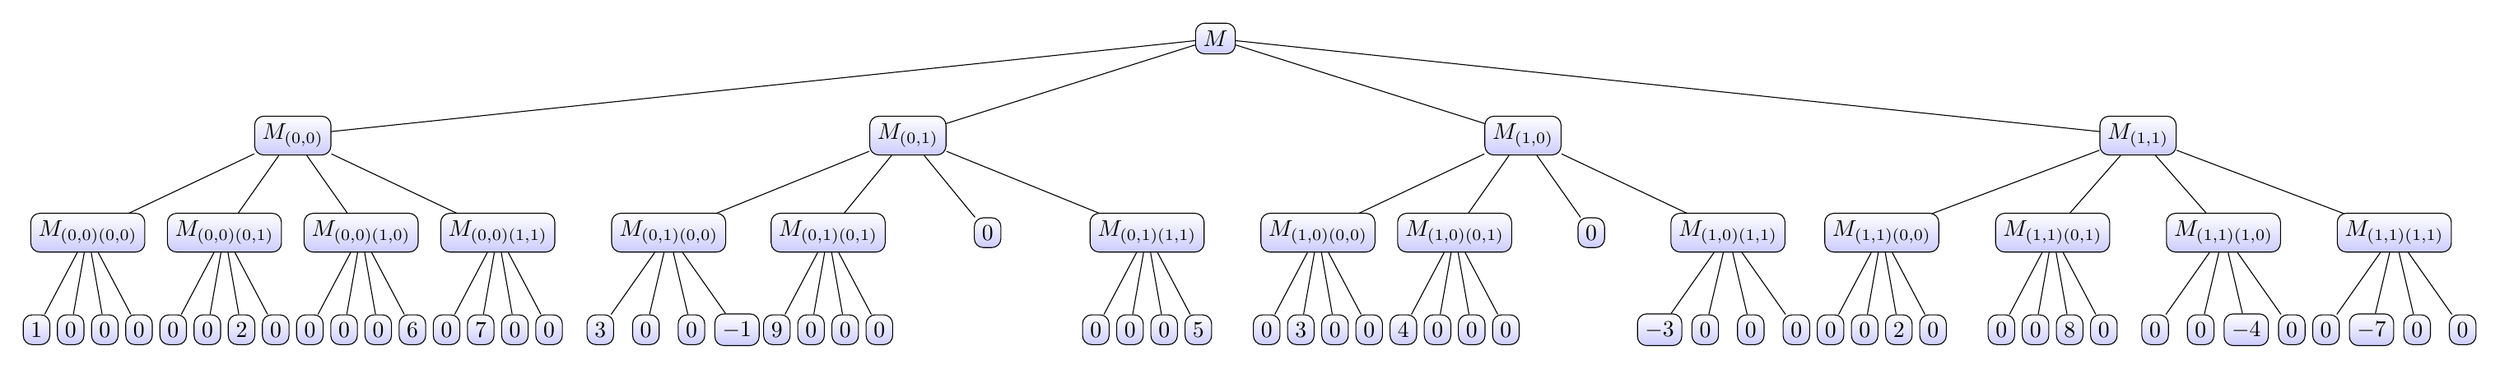
\begin{tikzpicture}[sibling distance=27em,
  every node/.style = {shape=rectangle, rounded corners,
    draw, align=center,
    top color=white, bottom color=blue!20}]
  \node {$M$}
    child {[sibling distance=6em]
        node {$M_{(0,0)}$}
        child { [sibling distance=1.5em]
            node {$M_{(0,0)(0,0)}$}
            child {node {$1$}}
            child {node {$0$}}
            child {node {$0$}}
            child {node {$0$}} }
        child { [sibling distance=1.5em]
            node {$M_{(0,0)(0,1)}$}
            child {node {$0$}}
            child {node {$0$}}
            child {node {$2$}}
            child {node {$0$}} }
        child { [sibling distance=1.5em]
            node {$M_{(0,0)(1,0)}$}
            child {node {$0$}}
            child {node {$0$}}
            child {node {$0$}}
            child {node {$6$}} }
        child { [sibling distance=1.5em]
            node {$M_{(0,0)(1,1)}$}
            child {node {$0$}}
            child {node {$7$}}
            child {node {$0$}}
            child {node {$0$}} } }
    child { [sibling distance=7em]
        node {$M_{(0,1)}$}
        child { [sibling distance=2em]
            node {$M_{(0,1)(0,0)}$}
            child {node {$3$}}
            child {node {$0$}}
            child {node {$0$}}
            child {node {$-1$}} }
        child { [sibling distance=1.5em]
            node {$M_{(0,1)(0,1)}$}
            child {node {$9$}}
            child {node {$0$}}
            child {node {$0$}}
            child {node {$0$}} }
        child { node {$0$} }
        child { [sibling distance=1.5em]
            node {$M_{(0,1)(1,1)}$}
            child {node {$0$}}
            child {node {$0$}}
            child {node {$0$}}
            child {node {$5$}} } }
    child { [sibling distance=6em]
        node {$M_{(1,0)}$}
        child { [sibling distance=1.5em]
            node {$M_{(1,0)(0,0)}$}
            child {node {$0$}}
            child {node {$3$}}
            child {node {$0$}}
            child {node {$0$}} }
        child { [sibling distance=1.5em]
            node {$M_{(1,0)(0,1)}$}
            child {node {$4$}}
            child {node {$0$}}
            child {node {$0$}}
            child {node {$0$}} }
        child { node {$0$} }
        child { [sibling distance=2em]
            node {$M_{(1,0)(1,1)}$}
            child {node {$-3$}}
            child {node {$0$}}
            child {node {$0$}}
            child {node {$0$}} } }
    child { [sibling distance=7.5em]
        node {$M_{(1,1)}$}
        child { [sibling distance=1.5em]
            node {$M_{(1,1)(0,0)}$}
            child {node {$0$}}
            child {node {$0$}}
            child {node {$2$}}
            child {node {$0$}} }
        child { [sibling distance=1.5em]
            node {$M_{(1,1)(0,1)}$}
            child {node {$0$}}
            child {node {$0$}}
            child {node {$8$}}
            child {node {$0$}} }
        child { [sibling distance=2em]
            node {$M_{(1,1)(1,0)}$}
            child {node {$0$}}
            child {node {$0$}}
            child {node {$-4$}}
            child {node {$0$}} }
        child { [sibling distance=2em]
            node {$M_{(1,1)(1,1)}$}
            child {node {$0$}}
            child {node {$-7$}}
            child {node {$0$}}
            child {node {$0$}} } };
\end{tikzpicture}
}
    \caption{Дерево квадрантов для матрицы $M$. Нулевые листья отмечены как $0$; в остальных листьях указано значение соответствующей ячейки.}
    \label{fig:QuadTree}
\end{figure}

Дерево квадрантов обладает несколькими привлекательными свойствами.
Рекурсивная структура позволяет легко разбивать матрицу на части, что удобно для распределённых вычислений.
Доступ к элементу выполняется за $O(k)$ шагов (спуск по дереву), где $k = \log_2 n$.
Перемножение матриц, представленных деревьями квадрантов, может быть реализовано рекурсивно, аналогично блочному умножению.
Недостатком является относительно высокая сложность построения по сравнению с <<плоскими>> форматами.

На практике часто применяются гибридные подходы: до некоторого уровня строится дерево квадрантов, а в его листьях хранятся сравнительно большие подматрицы, представленные в формате CSR или CSC.
Это позволяет сочетать преимущества иерархического и плоского представлений.

\paragraph{Разреженные вектора.}
К разреженным векторам применимы те же идеи, что и к разреженным матрицам, с учётом их одномерной природы.
Покоординатный формат для вектора вырождается в набор пар (индекс, значение).
Формат, аналогичный CSR, вырождается в два массива: массив значений и массив индексов (единственная <<строка>> или <<столбец>>).
В дальнейшем, при обсуждении матричных алгоритмов над разреженными структурами, разреженные вектора будут возникать как естественный частный случай.

Таким образом, выбор формата разреженной матрицы или вектора определяется конкретной задачей: частотой изменения данных, паттернами доступа и типом выполняемых операций.
Как мы увидим в главе~\ref{chpt:GraphTheoryIntro}, при анализе графов разреженные матрицы (в первую очередь~--- матрицы смежности) возникают повсеместно, и эффективная работа с ними является ключевым фактором производительности алгоритмов.
Детальное обсуждение прикладных аспектов~--- включая стандарт GraphBLAS и работу с неявными нулями~--- вынесено в раздел, посвящённый прикладным особенностям (там же, глава~\ref{chpt:GraphTheoryIntro}).
